\documentclass[12pt]{article}
\usepackage{graphics}
\usepackage[top=1in,bottom=1in,left=1in,right=1in]{geometry}
\usepackage{alltt}
\usepackage{array}	
\usepackage{graphicx}
\usepackage{tabularx}
\usepackage{verbatim}
\usepackage{setspace}
\usepackage{listings}

\usepackage{amssymb,amsmath, amsthm}
\usepackage{zed-csp}
\usepackage[cc]{titlepic}

\title{COMP 335: Introduction to Theoretical Computer Science\\
\ \\
Assignment 6}
\author{Nathan Grenier}
\date{\today \\ Fall 2024}

\begin{document}
\begin{spacing}{1.5}
      \maketitle

      \newpage

      \begin{enumerate}

            \item[1.] [30 Points] Classify the following languages into one of the three categories:
                  \begin{enumerate}
                        \item regular
                        \item context-free but not regular
                        \item not context-free
                  \end{enumerate}
                  Prove your answer. Note that in order to show that a language is context-free but not regular, you need to prove both that it is context-free and also that it is not regular.

                  \begin{enumerate}
                        \item[(a)] $L_1 = \{a^ib^jc^k | k=i\times j \text{ and } 0 < i < 10 < j\}$

                        \item[(b)] $L_2 = \{xyz | x,y,z \in \{a,b \}^* \text{ and } n_a(x)=n_b(z) \}$

                        \item[(c)] $L_3 = \{wuw^R | w,u \in \{a,b\}^* \text{ and } |w|=|u| \}$

                  \end{enumerate}

                  \newpage
            \item[2.] [10 Points] Give a Turing machine for $L=\{a \} \cdot \{a,b \}^+$ that does not halt on rejection.

                  % \begin{figure}[h!]
                  %       \centering
                  %       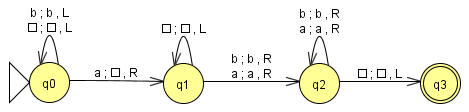
\includegraphics[width=0.5\textwidth]{img/q2/q2.png}
                  % \end{figure}

                  \newpage
            \item[3.] [20 Points] Give a Turing machine for each of the following languages.

                  \begin{enumerate}
                        \item[(a)] $L_1 = \{a^nb^mc^k | m \geq n, k \geq 1 \}$

                              % \begin{figure}[h!]
                              %       \centering
                              %       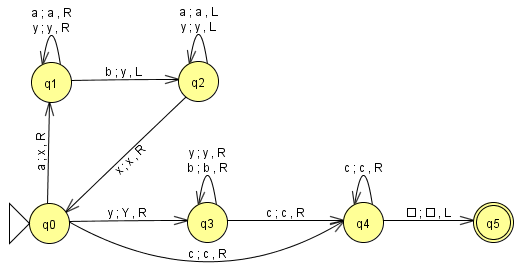
\includegraphics[width=0.5\textwidth]{img/q3/q3a.png}
                              % \end{figure}

                        \item[(b)] $L_2 = \{xy | x \in \{a,b \}^+, y \in \{c\}^+ \text{ and } n_a(x)=n_c(y) \}$

                              % \begin{figure}[h!]
                              %       \centering
                              %       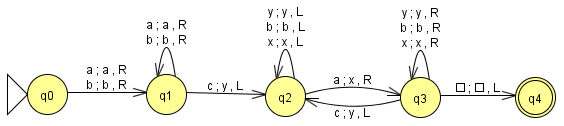
\includegraphics[width=0.5\textwidth]{img/q3/q3b.png}
                              % \end{figure}

                  \end{enumerate}

                  \newpage
            \item[4.] [20 Points] Draw transition diagrams for Turing machines that compute the following functions. In each case, give a brief description in English of your solution strategy.

                  \begin{enumerate}
                        \item[(a)] $f(1^n) = 1^{2n}$

                        \item[(b)] $f(1^n) = 1^{n^2}$

                  \end{enumerate}

      \end{enumerate}

\end{spacing}

\end{document}